\section{Research Object Management Tools}
\label{sec:romt}

This section presents the tools that we have developed for assisting users in creating and managing Research Objects. These tools are aimed towards different types of target users and needs and represent different levels of deployment of Wf4Ever RO management capabilities according to such requirements. RO Manager, myExperiment, and RODL comprise our portfolio of RO management tools for Wf4Ever's users (see figure~\ref{fig:romt}). Details from the exploitation point of view about such portfolio will be given in the final exploitation plan (deliverable D8.5v2) for Wf4Ever's project results.

The Research Object Manager (RO Manager, section~\ref{sec:romanager}) is a command line tool for creating, displaying and manipulating Research Objects, which incorporates the essential functionalities for RO management, especially by developers and in general a technically skilled audience used to working in a command-line environment. myExperiment (section~\ref{sec:myexperiment}) has been extended~\cite{DBLP:journals/fgcs/RoureGS09} to allow end-users, who are not necessarily information technology experts, to create, share, publish and curate workflow-centric Research Objects. The RO-enabled myExperiment incorporates a considerable amount of Wf4Ever's developments, especially the RO Model and Research Object management capabilities by its existing user-community. Finally, the Research Object Digital Library (RODL, section~\ref{sec:rodl}) acts as a full-fledged back-end not only for scientists but also for librarians and potentially other communities interested in the aggregation of heterogenous information sources with the rigor of digital libraries' best practices. While myExperiment is focused on workflow-centric Research Objects in scientific domains, RODL provides a holistic approach to the preservation of aggregated information sources and incorporates most of Wf4Ever's capabilities dealing with RO management, collaboration, versioning and evolution, and quality management. 


\begin{figure}
\begin{center}
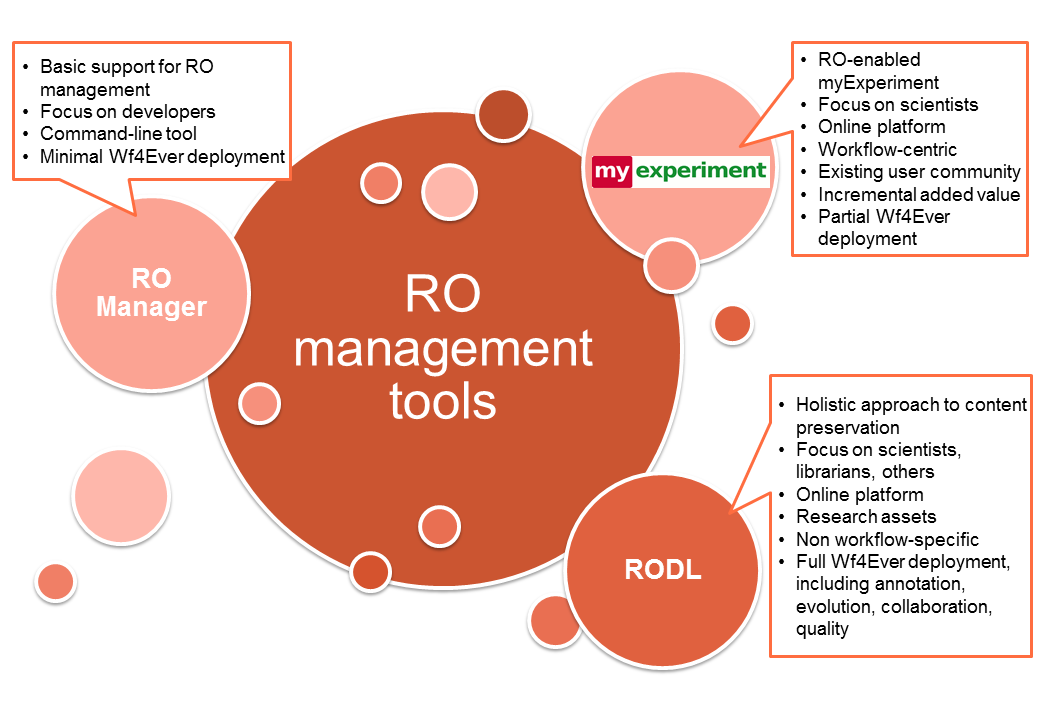
\includegraphics[width=0.85\textwidth]{Figures/ROManagementTools-exploitation.png}
\end{center}
\caption{Research Object management tools.}
\label{fig:romt}
\end{figure}